\chapter{Proposed Methodology}

The proposed methodology will be based on the frameworks proposed by Hoshyari, S., et. al. \cite{hoshyari2018perceptiondriven}, Yang, M., et. al. \cite{effectiveclipartimagevectorization}, Xiong, X., et. al. \cite{realtimevectorizationgpu}, and Laube, P., et. al. \cite{deeplearningparametrization}. Additionally, human perception will also be taken account. Thus, the Gestalt psychology principles of accuracy, simplicity, continuity, and closure, as taken from Hoshyari, S., et. al., will be taken into account as well.

\section{Image Preprocessing}
Before a raster input image can be fitted with curves, it must preprocessed to simplify the vectorization procedure and align it with .

\subsection{Corner Detection}
The first step in the approach is detecting the corners in the input image. This is an important step as it will allow us to enforce the simplicity principle in Gestalt psychology and make sure the resulting vectorization be C$^{0}$ continuous should the raster input be as such.

This stage will be based from the corner detection classifier of the work by Hoshyari, S., et. al. \cite{hoshyari2018perceptiondriven}. A random forest classifier is used in the said work. Supervised learning is used as corners are manually annotated. Annotated corners will not be specific pixels. Rather, corners will be between at least two pixels. Training data is available publicly provided by the researchers. However, such data is limited only to quantized data (i.e. aliased data). The target raster input is expected to be anti-aliased data. As such, the training data will have to be built from scratch to support anti-aliased data.

\subsection{Region Segmentation}
In line again with the simplicity principle, the input image must be divided into regions. This will result in simpler curves being used in the final vectorization output. The additional benefit of segmenting the input into multiple distinct regions is the possibility for parallelism to be used in the vectorization approach. Since each region is distinct and independent from one another, multiple regions can be vectorized at the same time. Thus, speeding up the vectorization process.

Due to the nature of semi-structured imagery where each region will only contain a single colour, a scanline-based approach can be used in this stage. The scanline algorithm will be based off of the scanline algorithm used for boundary pixel detection in the work of Xiong, X., et. al..

For each line $l_{i}$, where $0 \leq i < h \mid h$ is the height of input image, in the raster input, each pixel $p_{i}$ will be assigned to a pixel set $r_{ij}$, where $j$ is the index to a set in $l_{i}$. Each pixel set will contain horizontally adjacent pixels that have the same or near-same colours. We include pixels whose colours are within a certain threshold $k$ from the colour of the pixels that is most prominent in the set. This threshold is necessary due to the fact that certain parts of a regions may contain an anti-aliased pixel. Each $l_{i}$ will have a pixel set vector $r_{i}$ containing all pixel sets of $l_{i}$:

$$ r_{i} = (r_{i0}, r_{i1}, \ldots, r_{i(j - 1)}, r_{ij}) $$

Consequently, a region vector $r$ will contain all pixel set vectors.

$$ r = (r_{0}, \ldots, r_{i}) $$

Note that there is an opportunity to utilize parallelism, as shown in the work of Xiong, X., et. al. \cite{realtimevectorizationgpu}, during this step due to the independent nature of every line in the raster input.

Once we obtain all the pixel sets for each line, we iterate through $r$, ($h - 2$) times. For each iteration, we process $r_{i}$ and $r_{i + 1}$. If there are any $r_{ij_{\alpha}}$ whose pixels are vertically adjacent and have the same colour (or within $k$) to another pixel set $r_{(i + 1)j_{\beta}}$, then those two pixel sets are merged into one. By the end of the iterations, we have obtained a set of regions that we can individually vectorize.

\section{Curve Approximation}
The core step of the proposed approach is curve approximation. This stage fits curves to the region boundaries of the raster input. This stage is based on the work by Laube, P., et. al. on curve approximation on point sequences using deep learning \cite{deeplearningparametrization}.

\subsection{Point Sequence Generation}
The work of Laube, P., et. al. takes a point sequence as input. As such, for this proposed approach, we must generate point sequences from the region we will be vectorizing. For every region we ought to vectorize, we treat the center of boundary pixels and the detected corners of each region as a point sequence. However, we must also take into account the fact that certain portions of a region may be a corner where the curves in such segment would have C$_{0}$ continuity. As such, the point sequence we generate must take into account corners. This would implore us to take note of the following cases during point sequence generation:

\begin{enumerate}
	\item For regions with no corners, a random pixel will be selected as both start and end point of the point sequence. The expectation is that there will be no difference in the resulting curve from choosing a different start and end point.
	
	\item For regions with a single corner, the corner point will be selected as the start and end point of the point sequence. This is to ensure that the resulting vector output will have a corner at that point.
	
	\item For regions with two or more corners and assuming $n$ is the number of corners, the point sequence will be divided at those corners into separate point sequences. This will result in $(n + 1)$ new point sequences. Each new point sequence will have their start and end points be the corner points they are adjacent to.
\end{enumerate}

Each point sequence will then be passed to the next stage to be parametrized and have a curve approximated for.

\subsection{Point Sequence Curve Approximation}
The point sequences obtained from the previous step are now to be fitted with curves, specifically B-splines. As provided by the framework by Laube, P., et. al., two neural networks will be used in this stage and some preprocessing will be performed on the point sequences. The two neural networks are a point parametrization network (PPN), which approximates parametic values to point sequences, and a knot selection network (KSN), which predicts new knot values for knot vector refinement.

\subsubsection{Sequence Segmentation}
The input point sequence must first be split. This is to ensure that real data and training data match in terms of complexity. Let us define a function $\hat{k}(p)$ that measures the complexity of a point sequence $p$, where $k_{i}$ is the curvature at point $p_{i}$, given its total curvature:

$$ \hat{k}(p) = \sum_{i=0}^{m-1}\frac{(|k_{i}| + |k_{i + 1}|) \lvert\rvert  p_{i + 1} - p_{i} \lvert\rvert _{2}}{2} $$

A point sequence $p$ is split into point sequence segments $p^{s}, s = 1, \ldots, r$ at the median, if $\hat{k(p)} > \hat{k_{t}}$ for a threshold $\hat{k_{t}}$. This $\hat{k_{t}}$ will be set, as per the original authors have done, to the 98th percentile of $\hat{k}(\cdot)$ of the training set. This process is performed $r - 1$ times, until each $p^{s}$ satisfies $\hat{k(p)} > \hat{k_{t}}$.

\subsubsection{Sub/Supersampling and Normalization}
To be able to approximate parametric and knot values using the PPN and KSN, the number of points per segment $p^{s}$ must equal the input size $l$ of the aforementioned networks. As such, all segments $p^{s}$ are either subsampled or supersampled.

If a segment $p^{s}$ has a number of points greater than $l$, then $p^{s}$ is subsampled. This process involves drawing points in $p^{s}$ such that the drawn indices $i$ are equally distributed and include the first and last point. If, on the other hand, the number of points in $p^{s}$ is less than $l$, then \textit{temporary} points are linearly interpolated between consecutive points $p^{s}_{i}$ and $p^{s}_{i + 1}$. This interpolation is performed until the number of points equal $l$.

The sampled segments are then normalized to $\bar{p}^{s}$, which consists of the points

$$ \bar{p}^{s}_{i} = \frac{p^{s}_{i} - min(p^{s})}{max(p^{s}) - min(p^{s})} $$

where $min(p^{s})$ and $max(p^{s})$ are the minimum and maximum coordinates of $p^{s}$ respectively.

\subsubsection{Parametrization of Point Segments}

\begin{figure}[h]
	\centering
	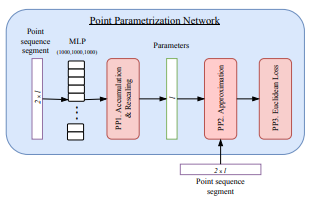
\includegraphics[scale=0.75]{images/chap05-methodology/ppn.png}
	\caption{The network architecture of the Point Parametrization Network (PPN)}.
	\label{fig:ppn}
\end{figure}

The PPN will be responsible for parametrization of point segments. For every $\bar{p}^{s}$, the PPN generates a parametrization $\bar{t}^{s} \subset [0, 1]$, which will be rescaled to $[u_{s - 1}, u_{s}]$ and adapted to sampling of $\bar{p}^{s}$.

In supersampled segments, the parameters $t^{s}_{i}$ of temporary points are simply removed from $\bar{t}^{s}$. In a subsampled $p^{s}$, for every point $p_{i}$ that was removed from the segment, a parameter $\bar{t}_{i}$ is inserted to $\bar{t}^{s}$.

$$ t_{i} = t^{s}_{\alpha} + (t^{s}_{\beta})\frac{chordlen(p^{s}_{\alpha}, p_{i})}{chordlen(p^{s}_{\alpha}, p^{s}_{\beta})} $$

$chordlen$ is the length of the polygon defined by a point sequence. In the subsampled segment, with parameters $t^{s}_{\alpha}$ and $t^{s}_{\beta}$, $p^{s}_{\alpha}$ and $p^{s}_{\beta}$ are the closest neighbours of $p_{i}$.

The initialization of the parametric step requires an initial knot vector. We first define $u_{0} = 0$ and $u_{n} = 1$. For each segment (except the last one), one knot $u_{i}$ is added.

$$ u_{i} = u_{i - 1)} + \frac{chordlen(p^{s})}{chordlen(p)}, i = 1, \ldots, r -1 $$
	
This yields a start and end knot for every point sequence segment.

\paragraph{The PPN Architecture}
The PPN, as stated earlier, takes in an input of segments $p$, which can be written as $p = (x_{0}, \ldots, x_{l - 1}, y_{0}, \ldots, y_{l - 1})$. The parameter domain is defined as $u_{0} = t_{0} = 0 and u_{n} = t_{l - 1} = 1$. For a sequence of points $p$, a parameter vector $t = (t_{i})_{i}$, is defined as $t_{i} = t_{i - 1} + \Delta_{i - 1}$. The task of the PPN is to predict missing values $\Delta = (\Delta_{0}, \ldots, \Delta_{l - 2})$ with

$$ \Delta_sub{i} > 0, i = 0, \ldots, l - 2 $$

such that $t_{0} < t_{1}$ and $t_{l - 2} < t_{l - 1}$. We apply a multilayer perceptron (MLP) to the input data $p$, yielding as output a distribution for parametrization $\Delta^{mlp} = (\Delta^{mlp}_{0}, \ldots, \Delta^{mlp}_{l - 2})$ of size $l - 1$.

The PPN further contains additional layers PP1, PP2, and PP3, which will be discussed next.

\subparagraph{PP1. Accumulation and Rescaling}
The output $\Delta^{mlp}$ is used to compute a parameter vector $t^{mlp}$ with $t^{mlp}_{0} = 0$ and

$$ t^{mlp}_{i} = \sum_{j = 0}^{i - 1}\Delta^{mlp}_{j}, i = 1, \ldots, l - 1 $$

Since $t^{mlp}_{l - 1}$ is usually not 1, rescaling $t^{mlp}$ yields the final parameter vector $t$ with

$$ t_{i} = \frac{t^{mlp}_{i}}{max(t^{mlp})} $$

The MLP layer in the PPN uses a softplus activation function defined to be:

$$ f(x) = ln(1 + e^{x}) $$

\subparagraph{PP2. Approximation}
B-spline curve approximation is included directly into the PPN as a network layer. The input points $p$ and their parameters $t$ are used for an approximation with knot vector $u = (0, 0, 0, 0, 1, 1, 1, 1)$ for $k = 3$. The approximation layer's output $p^{app} = (p^{app}_{0}, \ldots, p^{app}_{l - 1})$ is the approximating B-spline curve evaluated at $t$.

\subparagraph{PP3. Euclidean Loss}
A loss function, which is a Euclidean loss function, is to be used in the PPN. The Euclidean Loss function is defined as

\begin{equation}
\frac{1}{l}\sum_{i= 0}^{l - 1}\lvert\rvert p_{i} - p^{app}_{i} \lvert\rvert_{2} \label{eq:euclideanloss}
\end{equation}

\subsubsection{Parametrization Refinement}

\begin{figure}[h]
	\centering
	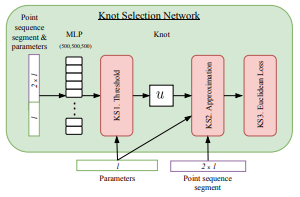
\includegraphics[scale=0.75]{images/chap05-methodology/ksn.png}
	\caption{The network architecture of the Knot Selection Network (PPN)}.
	\label{fig:ksn}
\end{figure}

In some cases, the approximated parametrization of a $p^{s}$ may have errors. The approximation error of a $p^{s}$ is computed by using the Hausdorff distance to the input data $p$.

The segments $p^{s}$ that have a large approximation error are computed a new knot using the KSN. For $\bar{p}^{s}$ and $\bar{t}^{s}$, the KSN generates a new estimated knot $\bar{u}_{s} \in [0, 1]$. The new knot $\bar{u}_{s}$ is mapped to the actual knot value range $[u_{s - 1}, u_{s}]$ by

$$ \tilde{u}_{s} = u_{s - 1} + \bar{u}_{s}(u_{s} - u_{s - 1}) $$

Instead of $\tilde{u}_{s}$, the parameter value $t_{i}$ closest to $\tilde{u}_{s}$ is inserted into $u$. $u$ can be further refined until the desired curve approximation error threshold is satisfied.

\paragraph{The KSN Architecture}
This stage utilizes a KSN, as mentioned earlier. The KSN predicts a new knot $u$ to the interval $(0, 1)$ for a given segment $p$ and parameters $t$, of which were previously approximated by the PPN. This network uses an MLP, which transforms the input to a single output value $u^{mlp}$. The RELU function is used as the activation function for the MLP, except for the output layer where the Sigmoid function is used instead.

Similar to that of the PPN, the KSN has three additional layers: KS1, KS2, and KS3.

\subparagraph{KS1. Threshold Layer}
The new knot $u$ computed has to satisfy the following conditions: $u \in (0, 1)$, $t \cap [0, u] \neq \theta$, and $t \cap [u, 1] \neq \theta$. Satisfying these conditions will will require us to use a threshold layer which maps $u^{mlp}$ to

$$ u = \begin{cases} \epsilon&\text{, if}\:u^{mlp} \le 0 \\ 1 - \epsilon&\text{, if}\:u^{mlp} \ge 1 \\ u^{mlp}&\text{, otherwise} \end{cases} $$

Introducing a small $\epsilon = 1e - 5$ makes sure that the knot multiplicity at the end knots stays equal to $k$.

\subparagraph{KS2. Approximation}
Approximation in the KSN is generally similar to that of PPN. The only different is that of the knot vector. The knot vector in the KSN is defined to be $u = (0, 0, 0, 0, u, 1, 1, 1, 1)$. For backpropagation, the derivative of the B-Spline basis functions with respect to $u$ is required.

\subparagraph{KS3. Euclidean Loss}
The loss function for the KSN is the same as that of the PPN. See \ref{eq:euclideanloss}.

\subsubsection{Network Training}
The training of the PPN and KSN will be based from the work of Laube, P., et. al. \cite{deeplearningparametrization}. The input size of the network will be $l = 100$.

The data set generated by the original authors consists of 150,000 curves. This data was synthesized from B-spline curves. Random control points $c_{i}$ were generated using a normal distribution $\mu$ and variance $\delta$ to define cubic ($k = 3$) B-spline curves with ($k + 1)$-fold end knots and no interior knots. The $y$-coordinates are given the configuration: $\delta = 2$ and $\mu = 10$. For the $x$-coordinates, $\delta = 1$ and $\mu = 10$ are used for the first control point. All consecutive points have $\mu$ increased by $\Delta\mu = 1$. Curves with self-intersections are discarded, because the sequential order of their sampled points is not unique, and point sequences are usually split into subsets at the self-intersections. Smaller $\delta$ for the x-coordinates of control points reduces the number of curves with self-intersections. To closely match the target input as much as possible, we also include curves that have been manually fitted to raster images. These curves can be obtained from vector images available online.

For each curve, $l$ points $p = (p_{0}, \ldots, p_{l - 1})$ are sampled. These curves then to have increasing x-coordinates from left to right. As such, index-flipped versions of the point sequences of the dataset are added, resulting in 300,000 point sequences. 20\% of the sequences are used as test data in the training process.

The PPN is trained first since the KSN requires point parametrizations $t$, which is obtained from the PPN. After training, the PP2 and PP3 layers are discarded and PP1 becomes the output layer of the PPN. The parametric values $t$ are computed for the training dataset by applying the PPN and train the KSN on the combined input. After training, KS2 and KS3 are discarded, with KS1 becoming the network output layer. The MLPs of the PPN and KSN will consist of three hidden layers with sizes (1000, 1000, 1000) and (500, 500, 500) respectively. Dropout is applied to the MLP layers. The network is trained using the Adam optimizer.

\section{Region Colouring and Merging}
Once the curves have been approximated, the vectorization of the region will be filled with the colour prominent in the raster version of the region. The regions will be plotted unto their locations in the original raster input. Once all the regions have been plotted, they will be grouped into a single vectorization. This will now be the vectorization output of the raster image.
 
%The input image will first be segmented into separate regions. At this point, the appropriate segmentation algorithm will be determined through experimentation. Notably, the separation of the regions will open up the possibility of using parallelism to speed up the execution of the algorithm.

%Once segmentation has been complete, each region will be applied corner detection. Corner detection will be performed using neural networks via supervised learning. The training data set will consist of anti-aliased input since the vectorization target will be anti-aliased input. A pre-vectorization of the curves, by connecting straight Bezier curves will connect the detected corners to one another.

%The final step will involve the optimization of the initial vectorization done during the pre-vectorization. The optimization framework will be based on the work by Yang, M.. The framework will be modified to include additional priors and weights To take into account Gestalt psychology.